\subsubsection{Antecedentes y Definición}
El desarrollo de las ontologías se deriva directamente de la filosofía, 
Aristóteles acuña el término ``Categoría'' como palabra para describir las
diferentes clases en las que se dividían las cosas del mundo. 
El término ``ontología'' es relativamente moderno (siglo XIX), proviene del griego
$Ontos$ (Ser) y $Logos$ (Palabra), se empezó a utilizar para diferenciar el
estudio de la Teoría de Categorías que se hacía en biología, de hecho, el trabajo de categorización surge en muchas áreas de la
ciencia (filosofía, biología, medicina, lingüística, etc.).

El cuerpo de un esquema de conocimiento, \textit{lo} que se puede representar, está basado en una
conceptualización: objetos, conceptos y otras entidades, que se asume existen en
un determinado dominio y que mantienen unas relaciones entre sí. 

\begin{Frame}
\textit{Una ontología es una especificación (explícita) de una conceptualización}~\cite{GruberOnto}. 
\end{Frame}

Las ontologías, por consiguiente, son sistemas basados en el conocimiento (\textit{\gls{SBC}}) que
sirven como modelo unificado en la representación del mismo, adquiriendo incluso
grado de ingeniería~\cite{isbn1846283965,Benjamins98ontological}. En muchos
casos, la Web Semántica y por extensión las ontologías se apoyan en la
reutilización de conocimiento compartido. Las definiciones realizadas para las ontologías son variadas y todas dejan claro
que sirven para modelar cierto dominio (conjunto de conceptos y relaciones):

\begin{itemize}
  \item Una ontología define los términos básicos y las relaciones establecidas en cierta área.
  \item Especificación explícita de una conceptualización.
  \item Especificación formal y explícita de una conceptualización compartida.
  \item Teoría lógica que provee de forma explícita y parcialmente una conceptualización.
  \item \ldots
\end{itemize}

En el artículo~\cite{Studer98knowledge} los autores agregan
expresividad realizando la siguiente descripción completa de ontología:
\begin{itemize}
  \item Conceptualización, modelo abstracto de algún fenómeno del mundo,
  proveniente de la identificación de los conceptos relevantes de dicho
  fenómeno. \item Explícita, conceptos y restricciones usados se definen
  explícitamente. \item Formal, capacidad de ser legible e interpretable por las
  máquinas.
  \item Compartida, captura conocimiento consensuado.
\end{itemize}

Es posible fusionar las definiciones anteriores en nueva descripción del término ontología:
\begin{definition}
Modelo conceptual organizado mediante una taxonomía que permite definir
relaciones entre conceptos, funciones, instancias (elementos) y axiomas en un determinado
dominio.
\end{definition}

Para completar la definición de ontología hay que tener en cuenta la
nomenclatura que habitualmente se utiliza para nombrar a las distintas entidades
posibles y que en algunos casos puede dar lugar a errores:

\begin{itemize}
  \item Clase, concepto, categoría o tipo.
  \item Instancia, individual.
  \item Entidad, objeto (clase o instancia).
  \item Propiedad, relación, slot, atributo, rol.
\end{itemize}

En la actualidad, la construcción de sistemas basados en conocimiento conlleva la
creación partiendo de cero de nuevas bases de conocimiento. La aspiración debería ser
utilizar componentes reutilizables~\cite{Gruber93towards}, de esta manera los desarrolladores deberían
crear sistemas con la agregación del conocimiento ya existente. El conocimiento definido, 
las técnicas de resolución de problemas y otros servicios, podrían ser
compartidos entre varios sistemas, impulsando la creación de grandes sistemas con
un bajo coste. Desde esta perspectiva, se pueden usar las ontologías como
infraestructura para sistemas ubicuos.

\subsubsection{Componentes}
Una ontología consta de un conjunto no vacío de conceptos identificados como
relevantes en el dominio a modelar, un conjunto de atributos para describir los
conceptos que pueden proveer de distintas fuentes: propios, heredados, etc., un
conjunto de funciones, un conjunto de axiomas que formalizan las condiciones que
deben cumplir los distintos conceptos y un conjunto de instancias o
realizaciones particulares de los conceptos.

\begin{description}
\item[Conceptos:] cualquier entidad que se puede describir, tiene asociado un
identificador único, puede poseer diferentes atributos y establecer relaciones
con otros conceptos.
\item[Relaciones:] representan la interacción entre los conceptos de dominio.
Formalmente, se definen como subconjuntos del producto cartesiano de $n$
conjuntos $R: C_1 \times C_2 \times \ldots \times C_n$.

No todas las relaciones tienen el mismo significado, existen relaciones binarias
de especialización como (\textit{is-a}) o de composición (\textit{part-whole}),
que se modelan con las propiedades clásicas simétricas, reflexivas, etc.

\item[Funciones:]relaciones en las cuales el elemento \textit{n-ésimo} es único para
los $n-1$ anteriores. Formalmente, se definen como $F:C_1 \times C_2 \times
\ldots \times C_n$. Por ejemplo una relación \textit{serPadreDe} se puede
modelar como una función ya que el atributo que evalúa es único para cada caso.

\item[Axiomas:] modelan ``verdades'' que siempre se cumplen en el modelo.
Existen dos tipos de axiomas:
\begin{itemize}
  \item Estructurales, condiciones relacionadas con la estructura jerárquica de
  la ontología. 
  \item No estructurales, establecen relaciones entre atributos de un concepto y
  son específicos de cada dominio.
\end{itemize}

\item[Instancias:] representan realizaciones específicas del dominio de la ontología.
\end{description}

\subsubsection{$Description Logics$ y ontologías}
\textit{Description Logics}~\cite{baader03description} (\gls{DL}s) son un conjunto de lógicas
formales en el área de \textit{Knowledge Representation}, utilizadas para la representación y
razonamiento del conocimiento en un dominio de forma no ambigua. Las DLs se
basan en una semántica perfectamente definida que provee un conjunto de
constructores y primitivas con un significado lógico preciso.

Los pilares de estas lógicas son dos conjuntos: uno de ellos, \textit{atomic concepts}
o predicados unarios y otro, \textit{atomic roles} o predicados binarios. Una
DL provee además un conjunto de operadores, llamados \textit{constructores}, que
permiten crear conceptos y roles más complejos a partir de los más sencillos.
Tanto los conceptos atómicos como los complejos, se denominan uniformemente \textit{conceptos}
y de igual forma, los roles atómicos y los complejos se denominan
\textit{roles}.

Los conceptos se utilizan para representar conjuntos de objetos y los roles
sirven para establecer relaciones binarias entre objetos. Podemos definir el
conjunto de los números reales como la disyunción de
números racionales e irracionales
\begin{example}
$ \mathbb{R} \equiv \mathbb{Q} \sqcup \mathbb{I}$
\end{example}

En general, una base de conocimiento basada en DL consiste en:
\begin{itemize}
  \item \textit{TBox}, contiene los axiomas de inclusión de conceptos
  $C_1 \sqsubseteq C_2$.
  \item \textit{RBox}, contiene los axiomas de inclusión de roles $R_1 
  \sqsubseteq R_2$.
  \item \textit{Abox}, contiene axiomas (aserciones sobre conceptos) $C(a)$, las
  aserciones sobre los roles $R(a,b)$, $a$ y $b$ son son nombre de objetos, $R$
  es un rol y $C$ es un concepto.
\end{itemize}
 
Los constructores booleanos de conceptos son la $\sqcup$ (disyunción o unión),
$\sqcap$ (conjunción o intersección) y $\neg$ (negación). Una
DL que provee, implícita o explícitamente, todos los operadores booleanos se
considera \textit{cerrada} (proposicionalmente). Las DLs ``cerradas'' serán las
que sean interesantes para su procesamiento en la Web Semántica. Aparte de los
operadores booleanos, habitualmente las DLs proveen otros constructores para
generar conceptos complejos a partir de roles. En este apartado, se encuentran
los operadores existencial ($\exists$)  y universal $\forall$. 

Las DLs que proveen estos cinco operadores se denominan $\mathcal{ALC}$, pero
esta lógica no permite axiomas de inclusión en roles y la componente 
\textit{RBox} es vacía, supone que si bien se pueden realizar operaciones
de razonamiento, la lógica a este nivel es poco expresiva. Añadiendo nuevos
constructores a $\mathcal{ALC}$ se obtiene el conjunto de lógicas
$\mathcal{ALC_{HR^+}}$ (también conocida como $\mathcal{SH}$), que resultan de añadir la
inclusión de axiomas (permitiendo diferentes tipos), sobre la \textit{RBox}.
Esta familia de lógicas, ver Tabla ~\ref{table:sh} extraída de~\cite{Cuenca}, es muy
interesante porque posee un gran poder expresivo y puede ser probada sobre razonadores DL, como FaCT++, Racer, Pellet o Hermit.


\begin{table}[htb]
\renewcommand{\arraystretch}{1.3}
\begin{center}
\begin{tabular}{|c|c|c|}
\hline
\textbf{Nombre constructor}&\textbf{Sintaxis}&\textbf{Lógica}\\
\hline
Concepto atómico& $A$ & \\
Concepto universal& $(\top)$ & \\
Rol atómico& $R$ & \\
Conjunción de conceptos& $C \sqcap D$ & \\
Disyunción de conceptos& $C \sqcup D$ & \\
Negación de concepto& $\neg C$ & \\
Restricción existencial& $\exists R.C$ & \\
Restricción universal& $\forall R.C$ & \\
Rol transitivo& $Trans(R)$ & $\mathcal{S}$\\
\hline
Jerarquía de roles& $R_1 \sqsubseteq R_2$ & $\mathcal{H}$\\
\hline
Inversión de roles& $(R^-)$ & $\mathcal{I}$\\
\hline
Nominales (instancias)& $\{o\}$ & $\mathcal{O}$\\
\hline
Restricciones funcionales de número& $\geq 2S  (\geq 1S)$ &
$\mathcal{F}$\\ \hline

Restricciones no cualificadas de número& $\geq nS  (\leq nS)$ &
$\mathcal{N}$\\ 

\hline

Restricciones cualificadas de número& $\geq nS.C  (\leq nS.C)$ &
$\mathcal{Q}$\\ 

\hline
\hline

\end{tabular}
\caption{Familia de lógicas $\mathcal{SH}$.}
\label{table:sh}
\end{center}
\end{table}

La lógica DL es importante para la construcción de ontologías ya que permite
construir bases de conocimiento formales, computables y no ambiguas. Aunque no siempre será indispensable este nivel 
de lógica, tanto para la descripción de dominios como para la Web Semántica, es necesario presentar y dar a conocer este conjunto
de lógicas, para así validar los modelos y mantener unos criterios
formales en la construcción de ontologías. Las ontologías construidas con lógica
DL proporcionan una base sólida para el desafío de la Web Semántica.


\subsubsection{Ontología como \textit{SBC}}
Como sistema basado en el conocimiento, ver Figura~\ref{fig:knowledge}, y teniendo en
cuenta la importancia de la utilización de \textit{Description Logics} como lógica para
la creación de ontologías, se pueden distinguir los tres componentes heredados de
la definición de \gls{DL}. Pero desde el punto de vista tanto del razonamiento como la
inferencia, operaciones importantes en cualquier \gls{SBC}, resultan de interés los
siguientes componentes: 1) \textit{Tbox}, parte terminológica (organizado jerárquicamente) o
conocimiento definido por intensión, consistente en conceptos, roles y construcciones más complejas por combinación de éstos y 
2) \textit{Abox} o parte extensional, es decir,  las afirmaciones sobre individuos``concretos''. Sobre estas dos componentes se podrá realizar
razonamiento, operación especialmente relevante para la Web Semántica, de dos formas:

\begin{description}
\item[Razonamiento \textit{Tbox}, intensional o estructural:] permite consultar la estructura de
conocimiento e inferir información a partir de ella. El mecanismo de
razonamiento estructural por excelencia es la subsunción de conceptos, permite
calcular todos los subconceptos a partir de un concepto dado o consultar si un concepto
es subconcepto de otro. Los razonamientos usuales en la \textit{Tbox} son: \begin{itemize} \item Consistencia, comprueba si el conocimiento tiene o no sentido. 
\item Subsunción, comprobación de sí todos los individuos que pertenecen a un concepto (el
subsumido) también pertenecen a otro concepto (el que subsume). \item 
Equivalencia, comprueba si dos clases denotan el mismo conjunto de instancias. \end{itemize}

Todos estos razonamientos son aplicables al problema de la satisfacibilidad de
fórmulas lógicas siempre que se utilice un lenguaje de definición de conceptos que
sea cerrado con respecto a la negación.

\item[Razonamiento \textit{Abox} o extensional:] permite inferir nuevas instancias a partir de las
definidas de forma explícita en la \textit{Abox}. Los razonamientos usuales en la \textit{Abox} son:
\begin{itemize}
\item Comprobación de instancias, verifica que un determinado individuo es una instancia de un concepto específico. 
\item  Consistencia de la base de conocimiento, implica verificar que cada
concepto que existe en la base de conocimiento admite, al menos, una instancia o
individuo. 
\item Realización, encuentra el concepto más
especifico del que un individuo es instancia.\end{itemize}

\end{description}

\begin{figure}[htb]
\centering
	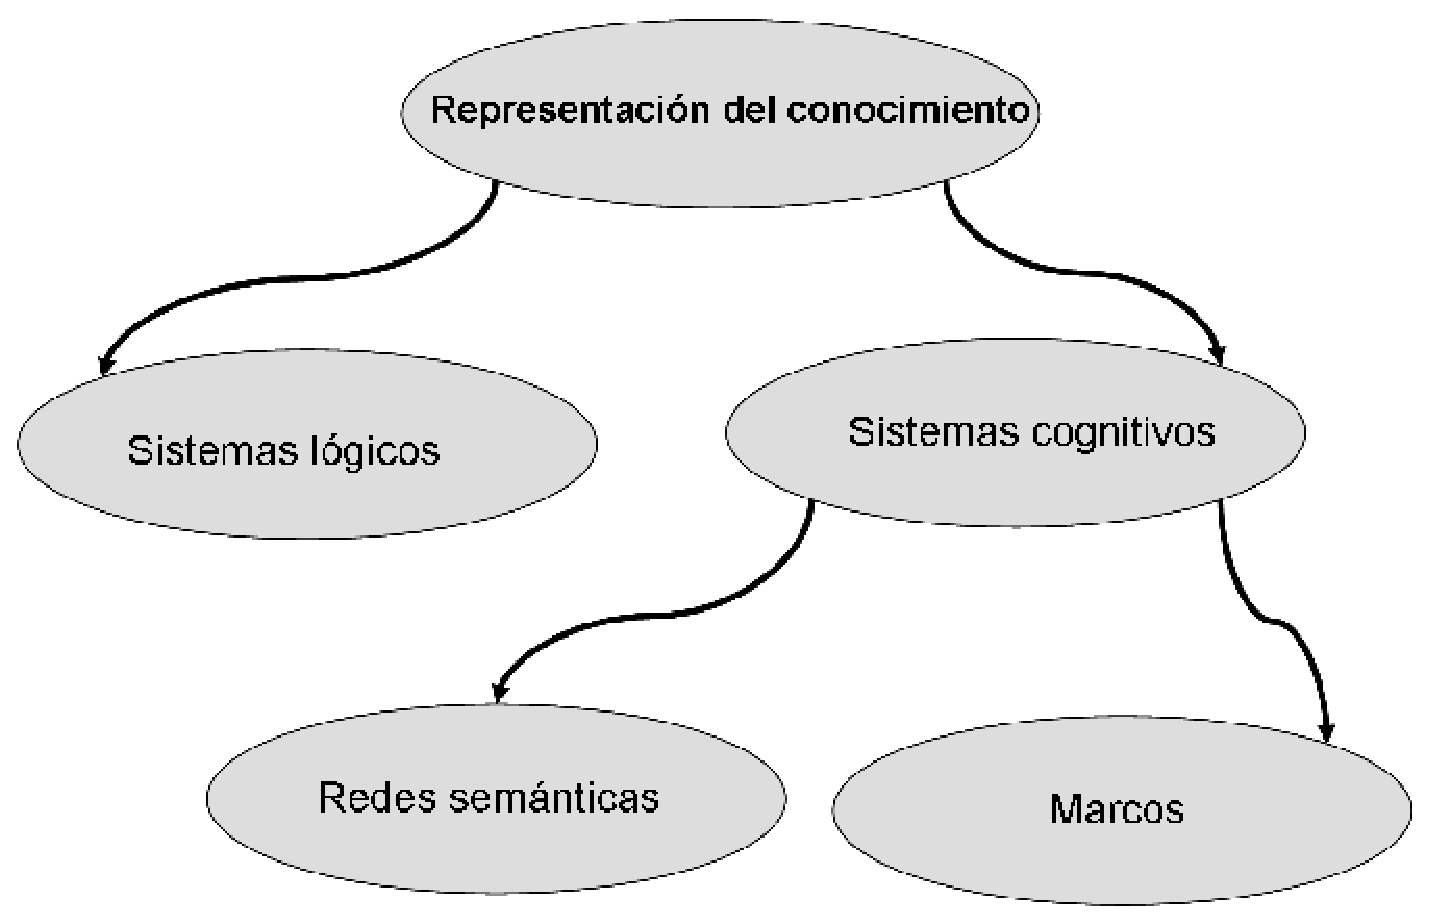
\includegraphics[width=10cm]{images/knowledge}
\caption{Sistemas basados en conocimiento.}
\label{fig:knowledge}
\end{figure}


\subsubsection{Clasificación de ontologías}
Las ontologías se pueden clasificar atendiendo a diferentes a criterios, a
continuación se exponen algunos de ellos.
\begin{description}
 \item [Grado de axiomatización.] Atendiendo a Sowa~\cite{Sowa99knowledge} las ontologías se pueden clasificar en:
\begin{description}
\item[Terminológicas:] define términos y sus relaciones en taxonomías que
involucran tanto relaciones de subtipo y supertipo, como las que relaciona
partes con un todo (\textit{part-whole}), no incluyen axiomas y definiciones
expresadas en lógica o lenguaje formal interpretable por una máquina. Por lo
tanto, existe menos información sobre el dominio modelado pero la simplicidad de
su especificación permite construir ontologías de gran tamaño.
\begin{example}
WordNet base de conocimiento (y datos) léxica.


Fuente: \url{http://wordnet.princeton.edu/}
\end{example}

\item[Formales:] consta de categorías restringidas por axiomas y definiciones
expresadas en alguna lógica formal, con menos conceptos pero preparadas para soportar
un procesamiento automático y servicios de razonamiento.

Una ontología terminológica podrá convertirse en formal a medida que se añadan
axiomas, aunque esta evolución no es ni mucho menos trivial.
\end{description}

\item[Según contexto.] Dependiendo del grado de dependencia del contexto las ontologías pueden ser:
\begin{description}
\item[Dominio:] modelan conceptualizaciones específicas, con restricciones de
estructura y contenido del dominio. Se reaprovecharán sólo en aquellas
aplicaciones que trabajen en ese dominio. Grado de dependencia alto.

\begin{example}
Ontología de medicina \textit{Galen}.


Fuente: \url{http://www.opengalen.org/}.
\end{example}

\item[Generales o de sentido común:] vocabularios o estructuras taxonómicas
genéricas. Alto grado de reaprovechamiento y bajo de dependencia del dominio.

\begin{example}
Cyc y OpenCyc.


Fuente: \url{http://www.cyc.com/}. 
\end{example}

\item[Metaontologías u ontologías genéricas:] ontologías de dominio genérico,
conceptos universales.
\begin{example}
DOLCE: Descriptive Ontology for Linguistic and Cognitive Engineering.


Fuente: \url{http://www.loa-cnr.it/DOLCE.html}. 
\end{example}

\end{description}

\item [Objeto de creación.]

Atendiendo al objetivo de creación de una ontología se establecen diferentes tipos:

\begin{itemize}
  \item Ontologías para la representación de conocimiento, como: \gls{OWL},
  \gls{DAML+OIL}, \gls{RDF}, RDF(S), OKBC, etc.
  \item Ontologías \textit{top level}, definen \textit{frameworks}, conceptos
  universales como las ya comentadas \textit{DOLCE} o \textit{Cyc}. 
  \item Ontologías para la definición de términos lingüisticos como
  \textit{WordNet} o \textit{EuroWordNet}~\cite{EuroWordNet}. 

	\item Ontologías de dominio, modelan conocimiento de cierto dominio: comercio
	electrónico o \textit{e-commerce}, de medicina \textit{Galen} o SNOMED, etc. 
\end{itemize}

\end{description}

Las ontologías como sistemas basados en conocimiento, serán más productivos
cuanto mejor ``informados'' estén, por ello, será interesante modelar utilizando
el mayor de grado de particularidad posible en el dominio, pero teniendo presente, que también es
importante mantener el objetivo de reutilizar conocimiento, podría ser interesante
enclavar los nuevos conceptos de dominio definidos dentro de las categorías de
alto nivel, para así alinear estas definiciones en un marco conceptual genérico.


\subsubsection{Principios de diseño}\label{onto-design}
Las ontologías deben o deberían cumplir una serie de principios:
\begin{description}
\item[Claridad:] proporcionar el significado pretendido a los términos
definidos. Definiciones tan objetivas como sea posible.
\item[Completitud:] las definiciones deberían recoger todas las condiciones
necesarias y suficientes, además de poseer una buena documentación en lenguaje natural.
 \item[Coherencia:] los términos definidos deben ser coherentes, concluyendo
 sólo aquellas inferencias consistentes con el modelo definido.
 \item[Extensibilidad:] anticipando la necesidad de reutilización y facilitando
 la adición de nuevo \linebreak conocimiento.
 \item[Mínimo compromiso ontológico:] minimizar el número de afirmaciones a
 realizar sobre el dominio modelado, permitiendo así que otros agentes las
 puedan refinar.

\item[Diversificación de jerarquías:] haciendo uso de la herencia múltiple, usar
tantos criterios de clasificación como sea posible. Así, añadir un nuevo concepto
es sencillo utilizando los ya existentes y la capacidad de clasificación.

\item[Minimizar la distancia semántica entre hermanos:] conceptos similares
deben agruparse.
 
  \item[Estandarización:] independencia simbólica, utilización de nombrado estándar.
 \item[Granularidad:] coherencia en el grado de particularidad, evitando el uso
 de términos ambig\"{u}os.
\end{description}

Finalmente, existen diversos procesos de desarrollo o metodologías que definen un
procedimiento para la captura de conocimiento de un dominio y la pertinente
construcción de ontologías. Por ejemplo: \textit{Methontology Framework} o \textit{Sensus method}. 


\subsubsection{Operaciones con ontologías}\label{op-ontologias}
En esta sección se describen las
operaciones~\cite{bruijn06-seman-web} que se pueden
realizar con las ontologías de acuerdo a su principio de reaprovechar el
conocimiento ya definido. La reutilización del conocimiento consensuado  es una de las
máximas de la creación de ontologías, para ello se definen tres operaciones
básicas (\textit{mapping} o correspondencia entre ontologías, \textit{merging} o
unión de ontologías y \textit{alignment} o descubrimiento de las
correspondencias de \textit{mapping} ) que
ayudan a la agregación de conocimiento basado en ontologías. La
importancia de estas operaciones se pone de manifiesto en la mediación de datos
entre fuentes heterogéneas, aspirando a resolver los conflictos que se producen
entre sistemas basados en conocimiento, que deben interaccionar entre sí pero que
han sido creados independientemente. El proceso de mediación, adquiere especial
interés para la propuesta de servicios web semánticos, en los cuales esta
operación es básica debido a la integración de ontologías provenientes de
diferentes modelos de negocio.  


\begin{description}
\item[\textit{Mapping} o \textit{mapeo} de ontologías:] especificación declarativa del
solapamiento semántico entre dos ontologías. Las correspondencias entre
entidades de ontologías diferentes son expresadas mediante axiomas en un
determinado lenguaje de \textit{mapeo}. Este proceso consta de tres fases: descubrimiento, representación y ejecución. Existen diferentes enfoques para llevar a cabo esta operación
como MAFRA, RDFT o C-OWL.
\item[\textit{Alignment} o alineamiento de ontologías:] proceso mediante el cual
se descubren las similitudes entre dos ontologías. El resultado es una especificación de los puntos en común, realizada a través del algoritmo 
\textit{Match operator}. Existen diferentes implementaciones como
Anchor-PROMPT, \linebreak GLUE, \textit{Semantic Matching} o QOM.
\item[\textit{Merging} o unión de ontologías:] creación de una ontología nueva
tomando como fuente dos o más ontologías. La nueva ontología unifica y reemplaza
las ontologías fuente. Se establecen dos enfoques para realizar esta
operación: 1) entrada de $n$ ontologías y salida de una sola
ontología, unión y reemplazo de las demás (por ejemplo: algoritmo
PROMPT~\cite{NM00}) y 2) entrada $n$ ontologías que no son reemplazadas, sino que se genera una ontología
\textit{bridge} que importa a las ontologías originales y especifica las correspondencias mediante
axiomas \textit{bridge}, por ejemplo \textit{OntoMerge}.
\end{description}

A la hora de afrontar la implementación de estas operaciones sobre ontologías se pueden generar dos tipos básicos de conflictos que impiden el éxito de la
operación y requieren intervención humana para facilitar la realización
automática de las operaciones: 
\begin{enumerate}
  \item Conflictos entre ``conceptualizaciones'' distintas del mismo dominio. A
  su vez, se distinguen dos categorías: 1) conflicto de ámbito, ocurre cuando dos clases tienen solapamiento en sus extensiones (el
  conjunto $s$ de instancias), y no coincide exactamente y 2) conflicto en la
  cobertura del modelo y su granularidad, ocurre si dos ontologías cubren parte
  de cierto dominio (por ejemplo: empleados de universidad y estudiantes) o bien
si una es más específica que otra (por ejemplo: una ontología define ``persona'' y otra define ``persona joven'').
  \item Conflictos entre las especificaciones de los conceptos. También, se diferencian tres categorías:\linebreak 1) conflicto en el estilo de
  modelado, cada ontología específica los conceptos de una manera determinada
(por ejemplo: tratamiento de las unidades de tiempo) o la descripción de los
conceptos   difiere (por ejemplo: utilización de subclases vs atributos); 2) conflicto
en la  terminología, dos conceptos son equivalentes pero no utilizan el mismo nombre,
  problema de sinónimos, o viceversa, son diferentes y utilizan el mismo nombre,
  homónimos y 3) conflicto de codificación, no se utilizan las mismas
  nomenclaturas, unidades de medida, etc.
\end{enumerate}

Todos estos conflictos, vienen en muchos casos provocados por no ajustarse a los
principios de diseño establecidos en la Sección~\ref{onto-design}. No
obstante, es habitual afrontar los problemas surgidos en la integración de ontologías ya que los
modeladores provienen de distintas partes, con diferente formación y puede que
sigan procedimientos particulares para la realización del modelado de
las ontologías, facilitando las tareas a las aplicaciones que las consuman.


\subsubsection{Aplicación de las ontologías}
Las ontologías se convierten en la pieza fundamental de ciertas áreas así pueden señalarse las 
siguientes:

\begin{description}
\item[Ingeniería del conocimiento:] las ontologías se pueden manifestar durante la ejecución de las siguientes tareas:
\begin{itemize}
  \item Construcción del modelo conceptual, generando los términos del glosario
  y de las relaciones que se establecen entre ellos.
  \item Construcción de la base de conocimiento, utilizando la ontología de
  modelado conceptual se pueden crear bases de conocimiento con la aplicación de
  reglas, restricciones, etc.
\end{itemize}

\item[Procesamiento del lenguaje natural:] mantenimiento de la definición de términos
gramaticales del lenguaje y las relaciones entre ellos.

\item[Integración de sistemas heterogéneos:] gestión de las diferencias
existentes entre diversos sistemas de información con el objetivo de facilitar
la comunicación entre los mismos.
\item[Búsqueda semántica:] utilizando conceptos y no términos para realizar las
búsquedas. 

\item[Web Semántica:] las ontologías son la base de la Web Semántica, por ello
cualquier aplicación que tenga un carácter semántico se apoyará, muy
probablemente, en ontologías.
\end{description}


Las ontologías se abren paso con fuerza sobre todo en el ámbito de las
aplicaciones~\cite{DBLP:conf/nldb/Penalver-MartinezVS11} de la Web Semántica, en particular en el escenario de la
integración de aplicaciones (servicios web semánticos~\cite{DBLP:journals/es/SanchezSMAVG11}) y contextualización del
usuario. En la construcción de una ontología, hay que afrontar el modelado desde el
punto de vista de la lógica (tipo y lenguaje de expresión) siguiendo los
principios de diseño, ver Sección~\ref{onto-design}, y no de la orientación a objetos, muy frecuente en el ámbito de la ingeniería del \textit{software}.  
